\documentclass[border=10pt]{standalone}

%draw
\usepackage{tikz}
\usepackage{pgfplots}
\usetikzlibrary{shapes.geometric, arrows}
\usetikzlibrary{arrows,automata}
\usetikzlibrary{arrows,positioning}
\usetikzlibrary{shapes.multipart}
% \pgfplotsset{compat=1.15}%        <--- added too

\begin{document}
    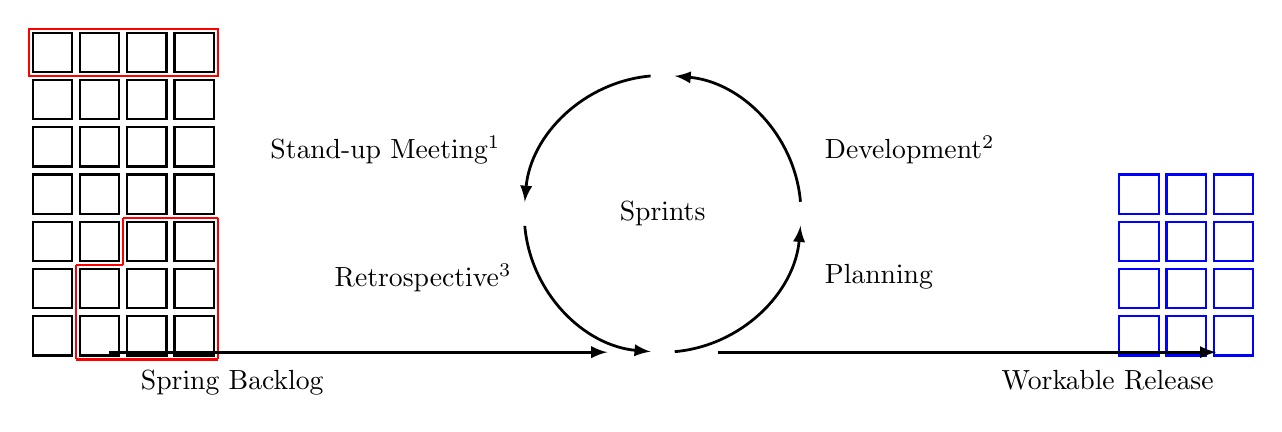
\begin{tikzpicture}[text centered]
        \foreach \x in {-8, -7.4, -6.8, -6.2}
        \foreach \y in {1.8, 1.2, ..., -2.4}
            \draw[thick] (\x,\y) rectangle (\x+0.5,\y+0.5);

        \foreach \x in {7, 6.4, 5.8}
        \foreach \y in {0, -0.6, -1.2, -1.8}
            \draw[blue, thick] (\x,\y) rectangle (\x+0.5,\y+0.5);

        %\draw[red, thick] (-7.45, -0.05) rectangle (-5.65, -1.85);
        \draw[red, thick] (-6.85, -0.05) -- (-5.65, -0.05);
        \draw[red, thick] (-5.65, -0.05) -- (-5.65, -1.85);
        \draw[red, thick] (-5.65, -1.85) -- (-7.45, -1.85);
        \draw[red, thick] (-7.45, -1.85) -- (-7.45, -0.65);
        \draw[red, thick] (-7.45, -0.65) -- (-6.85, -0.65);
        \draw[red, thick] (-6.85, -0.65) -- (-6.85, -0.05);
        \draw[red, thick] (-8.05, 2.35) rectangle (-5.65, 1.75);
        \node (sprints) {Sprints};

        \draw[->,latex-,line width=0.1em] (175:5em) node[above left=1em and 0.5em] {Stand-up Meeting\footnotemark} arc (175:95:5em);
        \draw[->,latex-,line width=0.1em] (85:5em) arc (85:5:5em) node[above right=1em and 0.5em] {Development\footnotemark};
        \draw[->,latex-,line width=0.1em] (265:5em) arc (265:185:5em) node[below left=1em and 0.1em] {Retrospective\footnotemark};
        \draw[->,latex-,line width=0.1em] (355:5em) node[below right=1em and 0.5em] {Planning} arc (355:275:5em);

        \draw[->,-latex,line width=0.1em] +(-20em,-5em) -- +(-2em,-5em);
        \draw[->,-latex,line width=0.1em] +(2em,-5em) -- +(20em,-5em);

        \node (start) [below left=4.5em and 10em of sprints] {Spring Backlog};
        \node (end) [below right=4.5em and 10em of sprints] {Workable Release};

    \end{tikzpicture}

\end{document}
